
\section{Results}

The model has been applied to two non-stationary environments.

\subsection{Zero-steps distribution shift}
In this first setting, as the end of a trial $i$ the arm distribution changes immediately to a new one $i+1$ as $\mathbf{\pi}_{i} \to \mathbf{\pi}_{i+1}$.

\begin{figure}[h]
    \centering
    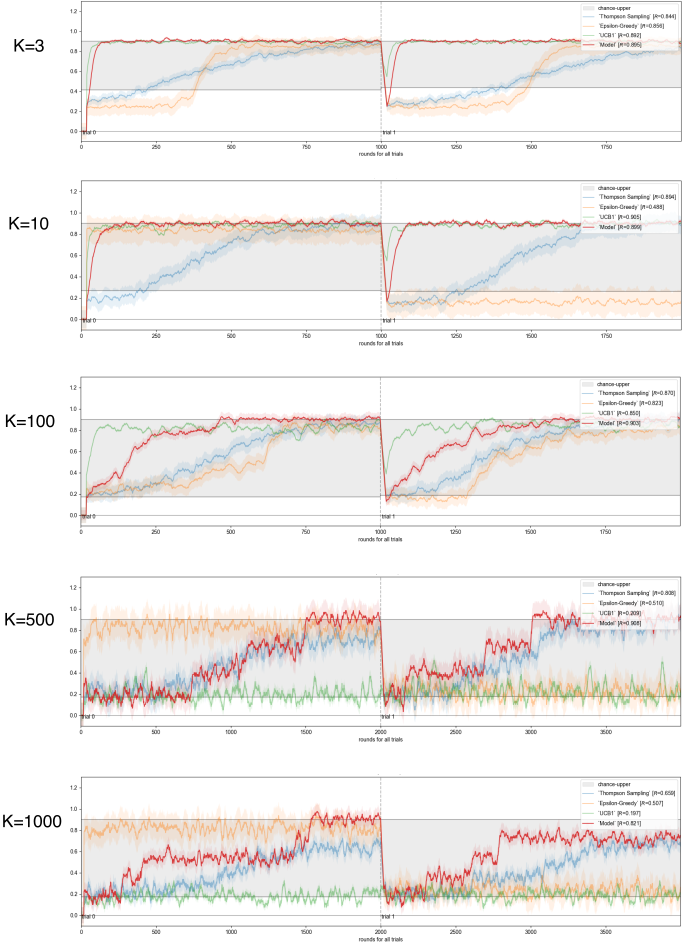
\includegraphics[width=0.65\textwidth]{figures/drawing.png}
    \caption{\textsc{Performance with variable number of arms} - \textit{each plot is an average of 50 simulations with K numbers of arms, the x-axis are rounds, the central vertical line signals the start of the second trial, the y-axis is the reward fraction.
            The shaded area is the reasonable reward
    range, where the lower bound is the chance level and the upper bound the best reward (following the optimal policy). The model performance is in red, while Upper-Confidence Bound green, Thompson Sampling blue, and Epsilon-Greedy orange. }}
\label{fig:zero_1}
\end{figure}


\noindent In Figure \ref{fig:zero_1} above, it is reported the average


\newpage
\subsection{Epsilon-steps distribution shift}

\begin{figure}[h]
    \centering
    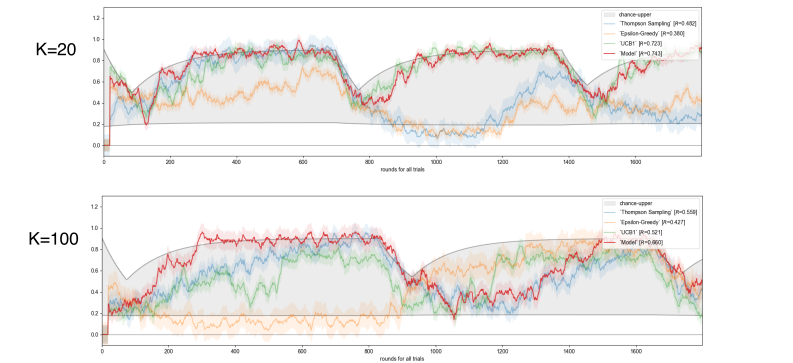
\includegraphics[width=0.8\textwidth]{figures/drawing2.png}
    \caption{\textsc{Performance with variable number of arms} - \textit{each plot is a simulation with K-numbers of arms, and the rest is also the same as before in \ref{fig:zero_1}}}
    \label{fig:eps_1}
\end{figure}

